\part{Lecture 02: Markov Decision Processes}
\title[RL Lecture 02]{Lecture 02: Markov Decision Processes}  
\date{}  
\frame{\titlepage} 

%%%%%%%%%%%%%%%%%%%%%%%%%%%%%%%%%%%%%%%%%%%%%%%%%%%%%%%%%%%%%
%% Preface / Motivation %%
%%%%%%%%%%%%%%%%%%%%%%%%%%%%%%%%%%%%%%%%%%%%%%%%%%%%%%%%%%%%%
\frame{\frametitle{Preface}
\begin{itemize}
	\onslide<2->\item Markov decision processes (MDP) are a \hl{mathematically idealized form of RL problems}.
	\onslide<2->\item They allow precise theoretical statements (e.g., on optimal solutions).
	\onslide<2->\item They deliver insights into suitable RL algorithms since many real-world problems can be abstracted as MDPs. 
	\onslide<3->\item In the following \hl{we'll focus on}:
	\onslide<3->\begin{itemize}
		\item fully observable MDPs (i.e., $\bm{x}_k=\bm{y}_k$) and 
		\item finite MDPs (i.e., finite number of states \& actions).
	\end{itemize}
\end{itemize}
\hfill
\onslide<1->\begin{table}
	\centering
		\begin{tabular}{|M{0.5cm}|M{1cm}||M{3cm}|M{3cm}|}
		\cline{3-4}
			\multicolumn{2}{c||}{\multirow{2}{*}{}}& \multicolumn{2}{c|}{All states observable?}\\
			\cline{3-4}
			\multicolumn{2}{c||}{} & Yes & No\\
			\hline\hline
			 \multirow{2}{*}{\rotatebox{90}{Actions?}} & No & Markov chain &Hidden Markov model\\
			\cline{2-4}
			& Yes & Markov decision process (MDP) & Partially observable MDP\\
			\hline
		\end{tabular}
	\caption{Different Markov models}
	\label{tab:DifferentMarkovModels}
\end{table}
}

%%%%%%%%%%%%%%%%%%%%%%%%%%%%%%%%%%%%%%%%%%%%%%%%%%%%%%%%%%%%%
%% Remark: Scalar and Vectorial State/Action Representation %%
%%%%%%%%%%%%%%%%%%%%%%%%%%%%%%%%%%%%%%%%%%%%%%%%%%%%%%%%%%%%%
\frame{\frametitle{Scalar and Vectorial Representations in Finite MDPs}
\begin{itemize}
	\onslide<1->\item The position of a chess piece can be represented in two ways:
	\begin{itemize}
		\onslide<1->\item Vectorial: $\bm{x}=\begin{bmatrix}x_h & x_v\end{bmatrix}\T$, i.e., a two-element vector with horizontal and vertical information (e.g., $\bm{x}=\begin{bmatrix}c & 1 \end{bmatrix}\T$) or
		\onslide<2->\item \hl{Scalar: simple enumeration of all available positions (e.g., $x=3$).}
	\end{itemize}
	\onslide<3->\item Both ways represent the same amount of information and can be easily converted into each other.
	\onslide<3->\item For sake of readability \hl{we will stick to the scalar representation of states and actions in finite MDPs} whenever possible.
\end{itemize}
\onslide<1->\begin{figure}		
	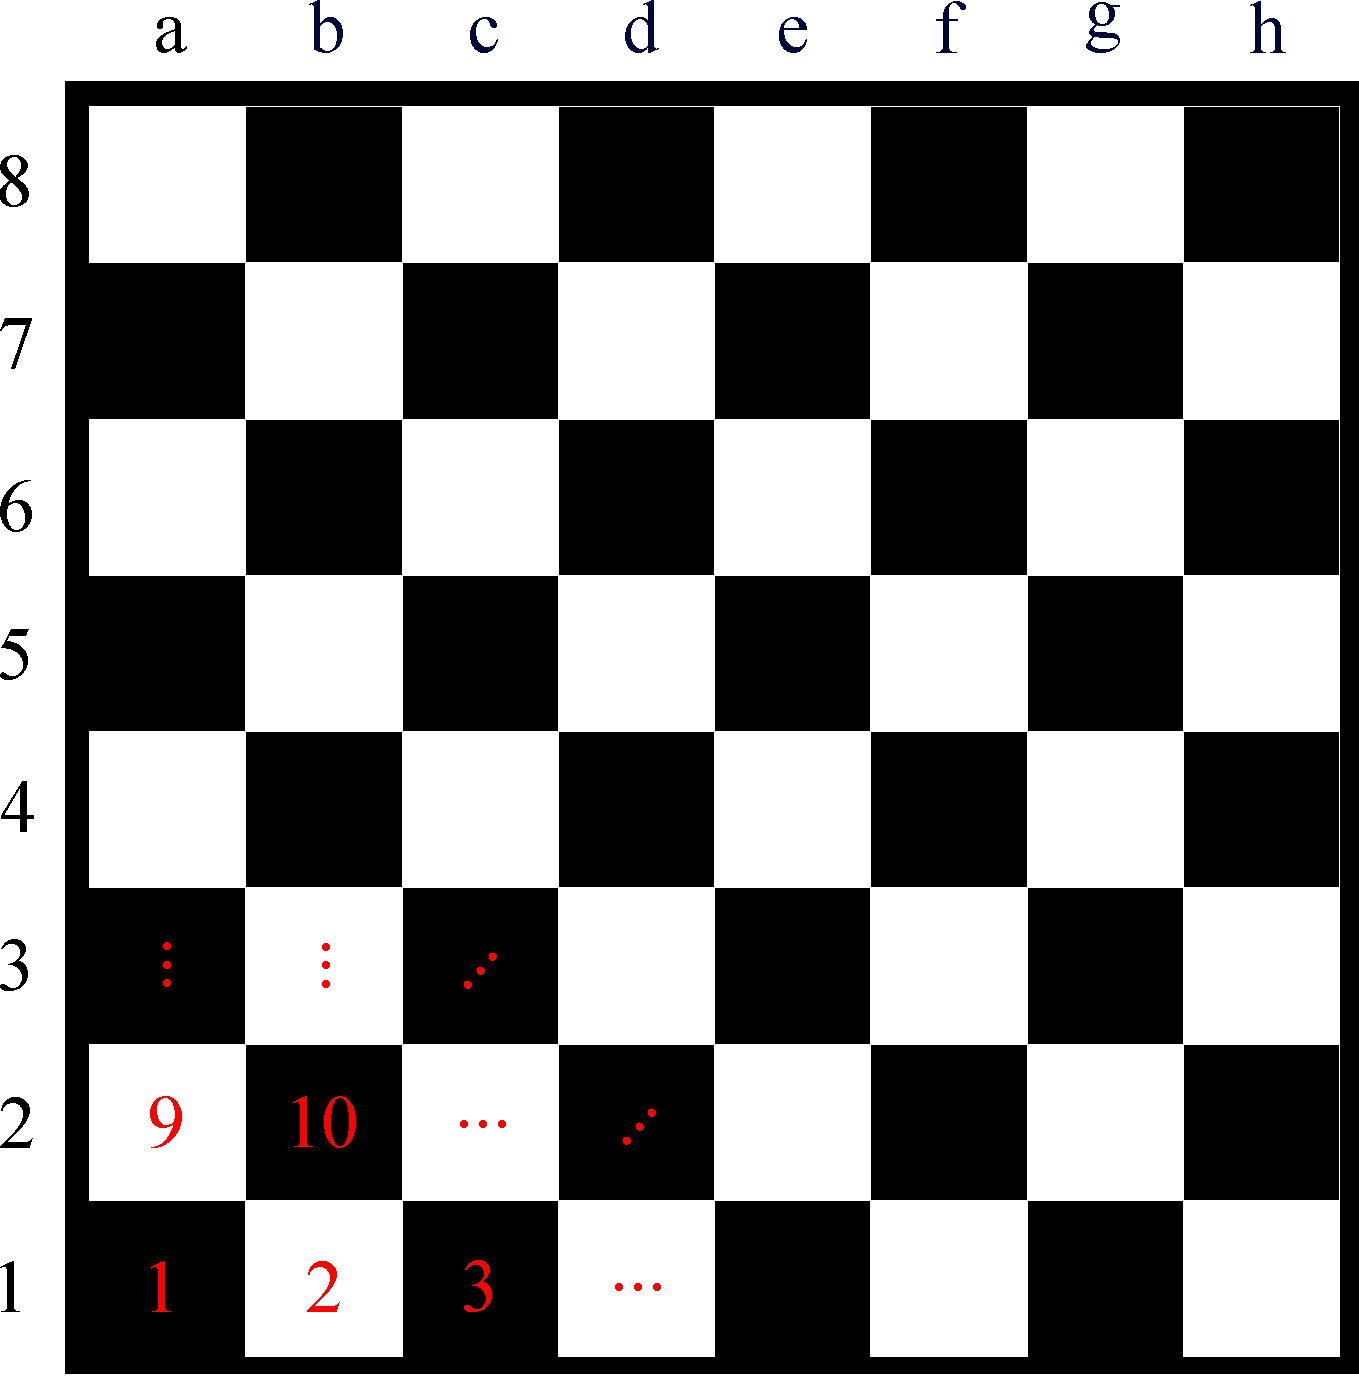
\includegraphics[width=4cm]{fig/lec02/Chess_Board.pdf}
\end{figure}
}

\frame{\frametitle{Table of Contents}\tableofcontents} 

%%%%%%%%%%%%%%%%%%%%%%%%%%%%%%%%%%%%%%%%%%%%%%%%%%%%%%%%%%%%%%%%%%
\section{Finite Markov Chains} 
%%%%%%%%%%%%%%%%%%%%%%%%%%%%%%%%%%%%%%%%%%%%%%%%%%%%%%%%%%%%%%%%%%

%%%%%%%%%%%%%%%%%%%%%%%%%%%%%%%%%%%%%%%%%%%%%%%%%%%%%%%%%%%%%
%% Recap Markov Property %%
%%%%%%%%%%%%%%%%%%%%%%%%%%%%%%%%%%%%%%%%%%%%%%%%%%%%%%%%%%%%%
\frame{\frametitle{Recap on Markov Property}

\begin{block}{Information state}
A state $X_k$ is called an information or Markov state if and only if
\begin{equation}
	\Pb{X_{k+1}|X_k}=\Pb{X_{k+1}|X_0, X_1,\ldots, X_k}\, .
\end{equation}
\end{block}
\pause
\begin{itemize}
	\item History is fully condensed in the sample $X_k$, i.e., $X_{k+1}$ is only depending on $X_k$.
	\item A given system can be fully described by $X_k$.
	\item Further past observations $X_{k-1},X_{k-2},\ldots$ are irrelevant.
\end{itemize}
}

%%%%%%%%%%%%%%%%%%%%%%%%%%%%%%%%%%%%%%%%%%%%%%%%%%%%%%%%%%%%%
%% State Transistion Matrix %%
%%%%%%%%%%%%%%%%%%%%%%%%%%%%%%%%%%%%%%%%%%%%%%%%%%%%%%%%%%%%%
\frame{\frametitle{State Transition Matrix}

\begin{defi}{State transition matrix}{STM}
Given a Markov state $X_k=x$ and its successor $X_{k+1}=x'$ , the \hl{state transition probability} $\forall \left\{x,x'\right\}\in \mathcal{X}$ is defined by the matrix
\begin{equation}
	\bm{\mathcal{P}}_{xx'}=\Pb{X_{k+1}=x'|X_{k}=x} .
\end{equation}
 \end{defi}
\pause
Here,  $\bm{\mathcal{P}}_{xx'}\in\mathbb{R}^{n\times n}$ has the form
\begin{equation*}
	\bm{\mathcal{P}}_{xx'} = \begin{bmatrix} p_{11} & p_{12} & \cdots & p_{1n}\\ p_{21} &  &  & \vdots\\ \vdots & & & \vdots\\ p_{n1} & \cdots & \cdots & p_{nn}\end{bmatrix}
\end{equation*}
with $p_{ij}\in\left\{\mathbb{R}|0 \leq p_{ij} \leq 1 \right\}$ being the specific probability to go from state $x=X_i$ to state $x'=X_j$. Obviously, $\sum_{j} p_{ij}=1 \, \forall i$ must hold.
}

%%%%%%%%%%%%%%%%%%%%%%%%%%%%%%%%%%%%%%%%%%%%%%%%%%%%%%%%%%%%%
%% Markov Chain %%
%%%%%%%%%%%%%%%%%%%%%%%%%%%%%%%%%%%%%%%%%%%%%%%%%%%%%%%%%%%%%
\frame{\frametitle{Markov Chain}

\onslide<1->\begin{defi}{Finite Markov chain}{Markov_chain}
A \hl{finite Markov chain} is a tuple $\left\langle\mathcal{X}, \bm{\mathcal{P}} \right\rangle$ with
\begin{itemize}
	\item $\mathcal{X}$ being a finite set of discrete-time states $X_k\in\mathcal{X}$, 
	\item $\bm{\mathcal{P}}=\bm{\mathcal{P}}_{xx'}=\Pb{X_{k+1}=x'|X_{k}=x}$ is the state transition probability.
\end{itemize}
\end{defi}
\begin{itemize}
	\onslide<2->\item Specific stochastic process model
	\onslide<2->\item Sequence of random variables $X_k, X_{k+1},\ldots$
	\onslide<2->\item 'Memoryless'
	\onslide<3->\item In continuous-time framework: Markov process\only<3->{\footnote[1]{However, this results in a literature nomenclature inconsistency with Markov decision/reward 'processes'.}} 
\end{itemize}
}

%%%%%%%%%%%%%%%%%%%%%%%%%%%%%%%%%%%%%%%%%%%%%%%%%%%%%%%%%%%%%
%% Chapman–Kolmogorov Equation %%
%%%%%%%%%%%%%%%%%%%%%%%%%%%%%%%%%%%%%%%%%%%%%%%%%%%%%%%%%%%%%
\frame{\frametitle{Chapman-Kolmogorov Equation}
Define $\bm{p}_k\in\mathbb{R}^n$ as a \hl{probability row vector} where $p_{i,k}$ gives the probability of being in state $X_k \in\mathcal{X}$ at time-step $k$.  
\begin{defi}{Chapman-Kolmogorov equation for finite Markov chains}{Chapman_Kolmogorov_Equation}
The probability of being in state $X_{k+m}$ at time-step $(k+m)$ starting from state $x_{k}$ is given by:
\begin{equation}
	\bm{p}_{k+m} = \bm{p}_{k}\bm{\mathcal{P}}_{xx'}^{m} .
\end{equation}
\end{defi}
\pause
Hence, for $m\rightarrow\infty$ ('\textit{steady state}') the following equation must hold:
\begin{equation}
	\bm{p} = \bm{p}\bm{\mathcal{P}}_{xx'} .
	\label{eq:Chapman_steady}
\end{equation}
Solving \eqref{eq:Chapman_steady} for $\bm{p}$ given the transition probability $\bm{\mathcal{P}}_{xx'}$ gives insights which states of the Markov chain are visited in the long-run.
}


%%%%%%%%%%%%%%%%%%%%%%%%%%%%%%%%%%%%%%%%%%%%%%%%%%%%%%%%%%%%%
%% Forest Markov Chain Example (1)%%
%%%%%%%%%%%%%%%%%%%%%%%%%%%%%%%%%%%%%%%%%%%%%%%%%%%%%%%%%%%%%
\frame{\frametitle{Example of a Markov Chain (1)}
\begin{minipage}[t]{0.53\linewidth}
		\vspace{0pt}
		\begin{figure}		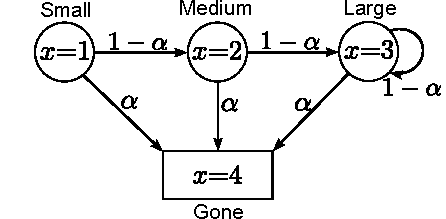
\includegraphics[width=6cm]{fig/lec02/Forest_Markov_Chain.pdf}
		\caption{Forest tree Markov chain}
		\label{fig:Forest_Markov_Chain}
	\end{figure}
\end{minipage}
\begin{minipage}[t]{0.45\linewidth}
\vspace{-0.7cm}
\begin{align*}
  x &= x\in\left\{1,2,3,4\right\}\\
				 &=\left\{\mbox{small},\mbox{medium},\mbox{large},\mbox{gone}\right\}\\[1em]
	\bm{\mathcal{P}} &= \begin{bmatrix}0 & 1-\alpha & 0 & \alpha  \\ 0 & 0 &1-\alpha & \alpha \\ 0 & 0 &1-\alpha & \alpha \\ 0 & 0 & 0 & 1\end{bmatrix}
\end{align*}
\end{minipage}
\begin{itemize}
	\item At $x=1$ a small tree is planted ('starting point').
	\item A tree grows with $(1-\alpha)$ probability.
	\item If it reaches $x=3$ (large) its growth is limited.
	\item With $\alpha$ probability a natural hazard destroys the tree.
	\item The state $x=4$ is terminal ('infinite loop').
\end{itemize}
}

%%%%%%%%%%%%%%%%%%%%%%%%%%%%%%%%%%%%%%%%%%%%%%%%%%%%%%%%%%%%%
%% Forest Markov Chain Example (2)%%
%%%%%%%%%%%%%%%%%%%%%%%%%%%%%%%%%%%%%%%%%%%%%%%%%%%%%%%%%%%%%
\frame{\frametitle{Example of a Markov Chain (2)}
\begin{figure}		
	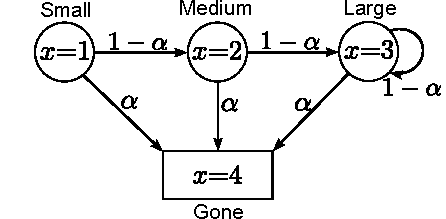
\includegraphics[width=6cm]{fig/lec02/Forest_Markov_Chain.pdf}
\end{figure}
Possible \hl{samples} for the given Markov chain example starting from $x=1$ (small tree):
\begin{itemize}
	\item Small $\rightarrow$ gone
	\item Small $\rightarrow$ medium $\rightarrow$ gone
	\item Small $\rightarrow$ medium $\rightarrow$ large $\rightarrow$ gone
	\item Small $\rightarrow$ medium $\rightarrow$ large $\rightarrow$ large $\rightarrow\ldots$ 
\end{itemize}
}

%%%%%%%%%%%%%%%%%%%%%%%%%%%%%%%%%%%%%%%%%%%%%%%%%%%%%%%%%%%%%
%% Forest Markov Chain Example (3)%%
%%%%%%%%%%%%%%%%%%%%%%%%%%%%%%%%%%%%%%%%%%%%%%%%%%%%%%%%%%%%%
\frame{\frametitle{Example of a Markov Chain (3)}
For $k=0$ the initial state probability is given $\bm{p}_{k=0}=\begin{bmatrix} 1 & 0 & 0 & 0\end{bmatrix}$, i.e., we are in state $x=1$. What is the state probability after $k=1,2,\ldots$ steps with $\alpha = 0.2$?
\begin{alignat*}{2}
	\onslide<2->{\bm{p}_{1}&=\begin{bmatrix}0 & 0.8 & 0 & 0.2\end{bmatrix}&&=\underbrace{\begin{bmatrix} 1 & 0 & 0 & 0\end{bmatrix}}_{\bm{p}_{0}}\underbrace{\begin{bmatrix}0 & 0.8 & 0 & 0.2  \\ 0 & 0 &0.8 & 0.2 \\ 0 & 0 &0.8 & 0.2 \\ 0 & 0 & 0 & 1\end{bmatrix}}_{\bm{\mathcal{P}}}},\\
	\onslide<3->{\bm{p}_{2}&=\begin{bmatrix}0 & 0 & 0.64 & 0.36\end{bmatrix}&&=\underbrace{\begin{bmatrix} 0 & 0.8 & 0 & 0.2\end{bmatrix}}_{\bm{p}_{1}}\underbrace{\begin{bmatrix}0 & 0.8 & 0 & 0.2  \\ 0 & 0 &0.8 & 0.2 \\ 0 & 0 &0.8 & 0.2 \\ 0 & 0 & 0 & 1\end{bmatrix}}_{\bm{\mathcal{P}}}},\\
	\onslide<4->{\bm{p}_{3}&=\begin{bmatrix}0 & 0 & 0.51 & 0.49\end{bmatrix}, &&\quad \bm{p}_{10}=\begin{bmatrix}0 & 0 & 0.11 & 0.89\end{bmatrix},\\
	\bm{p}_{\infty}&=\begin{bmatrix}0 & 0 & 0 & 1\end{bmatrix}.}
\end{alignat*}

}



%%%%%%%%%%%%%%%%%%%%%%%%%%%%%%%%%%%%%%%%%%%%%%%%%%%%%%%%%%%%%%%%%%
\section{Finite Markov Reward Processes} 
%%%%%%%%%%%%%%%%%%%%%%%%%%%%%%%%%%%%%%%%%%%%%%%%%%%%%%%%%%%%%%%%%%
\begin{frame}
\frametitle{Table of Contents}
\tableofcontents[currentsection]
\end{frame}

%%%%%%%%%%%%%%%%%%%%%%%%%%%%%%%%%%%%%%%%%%%%%%%%%%%%%%%%%%%%%
%% Markov Reward Process %%
%%%%%%%%%%%%%%%%%%%%%%%%%%%%%%%%%%%%%%%%%%%%%%%%%%%%%%%%%%%%%
\frame{\frametitle{Markov Reward Process}

\begin{defi}{Finite Markov reward process}{Markov_reward_process}
A \hl{finite Markov reward process (MRP)} is a tuple $\left\langle\mathcal{X}, \bm{\mathcal{P}}, \hl{\mathcal{R}, \gamma} \right\rangle$ with
\begin{itemize}
	\item $\mathcal{X}$ being a finite set of discrete-time states $X_k\in\mathcal{X}$, 
	\item $\bm{\mathcal{P}}=\bm{\mathcal{P}}_{xx'}=\Pb{X_{k+1}=x'|X_{k}=x}$ is the state transition probability,
	\item \hl{$\mathcal{R}$ is a reward function, $\mathcal{R}=\mathcal{R}_x=\E{R_{k+1}|X_k=x_k}$ and} 
	\item \hl{$\gamma$ is a discount factor, $\gamma\in\left\{\mathbb{R}|0 \leq \gamma \leq 1\right\}$}.
\end{itemize}
\end{defi}
\pause
\begin{itemize}
	\item Markov chain extended with rewards \pause
	\item Still an autonomous stochastic process without specific inputs \pause
	\item Rewards $R_k$ only dependent on state $X_k$
\end{itemize}
}

%%%%%%%%%%%%%%%%%%%%%%%%%%%%%%%%%%%%%%%%%%%%%%%%%%%%%%%%%%%%%
%% Forest Markov Reward Process %%
%%%%%%%%%%%%%%%%%%%%%%%%%%%%%%%%%%%%%%%%%%%%%%%%%%%%%%%%%%%%%
\frame{\frametitle{Example of a Markov Reward Process}
\begin{figure}		
	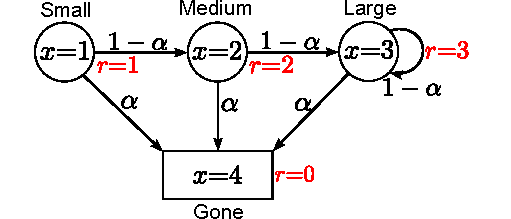
\includegraphics[width=10cm]{fig/lec02/Forest_Markov_Reward_Process.pdf}
	\caption{Forest Markov reward process}
	\label{fig:Forest_Markov_Reward_Process}
\end{figure}

\begin{itemize}
	\item Growing larger trees is rewarded, since it will be
	\begin{itemize}
		\item appreciated by hikers and
		\item useful for wood production.
	\end{itemize}
	\item Loosing a tree due to a hazard is unrewarded.
\end{itemize}
}

%%%%%%%%%%%%%%%%%%%%%%%%%%%%%%%%%%%%%%%%%%%%%%%%%%%%%%%%%%%%%
%% Recap Return %%
%%%%%%%%%%%%%%%%%%%%%%%%%%%%%%%%%%%%%%%%%%%%%%%%%%%%%%%%%%%%%
\frame{\frametitle{Recap on Return}

\begin{block}{Return}
The return $G_k$ is the total discounted reward starting from step $k$ onwards. For \hl{episodic tasks} it becomes the finite series
\begin{equation}
	G_k = R_{k+1} + \gamma R_{k+2} + \gamma^2 R_{k+3} + \cdots = \sum_{i=0}^N \gamma^i R_{k+i+1}  	
\end{equation}
terminating at step $N$ while it is an infinite series for \hl{continuing tasks}	
\begin{equation}
	G_k = R_{k+1} + \gamma R_{k+2} + \gamma^2 R_{k+3} + \cdots = \sum_{i=0}^\infty \gamma^i R_{k+i+1}\, .  	
\end{equation}
\end{block}
\begin{itemize}
	\item The discount $\gamma$ represents the value of future rewards.
\end{itemize}
}

%%%%%%%%%%%%%%%%%%%%%%%%%%%%%%%%%%%%%%%%%%%%%%%%%%%%%%%%%%%%%
%% Remark on notation: Episodic and Continuing Tasks %%
%%%%%%%%%%%%%%%%%%%%%%%%%%%%%%%%%%%%%%%%%%%%%%%%%%%%%%%%%%%%%
\frame{\frametitle{Remark on Notation: Episodic and Continuing Tasks}
\begin{itemize}
	\item In episodic tasks there is not only one (long/infinite) sequence of time steps.
	\item Instead there is a sequence of time steps of an arbitrary episode $j$.
	\begin{itemize}
		\item Formally: $X_{k,j},U_{k,j}, R_{k,j},\ldots$ 
	\end{itemize}
	\onslide<2->{
	\item Nevertheless, to increase the readability the episode index is normally dropped in this course:
	\begin{itemize}
		\item Simplified: $X_{k}\leftarrow X_{k,j},U_{k}\leftarrow U_{k,j}, R_{k}\leftarrow R_{k,j},\ldots$ 
	\end{itemize}
	\item Only in certain cases the episode indexing will be re-activated.
\end{itemize}}
\begin{figure}
	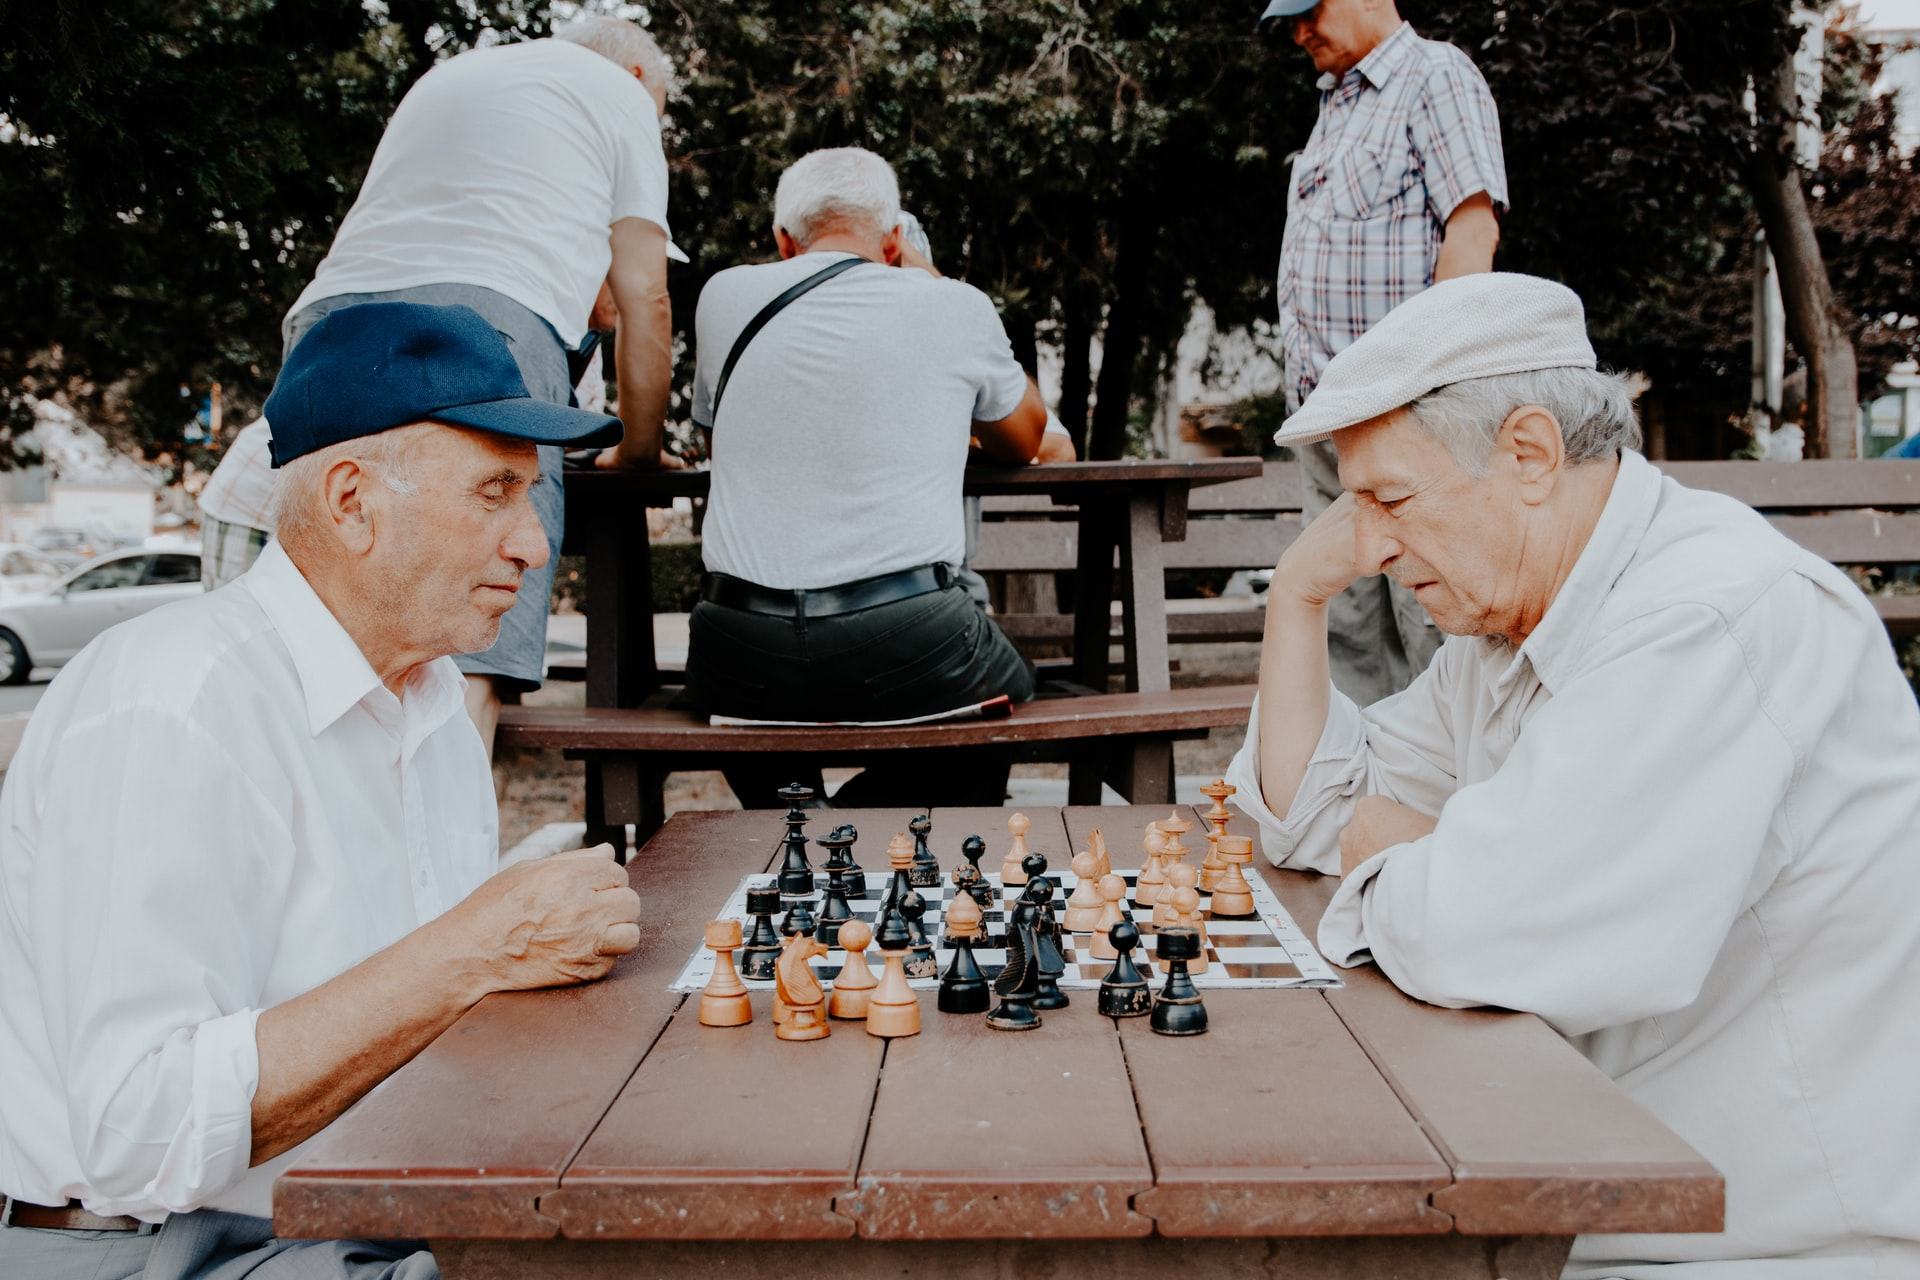
\includegraphics[width=5.5cm]{fig/lec02/chess_elderly_men.jpg}
	\caption{RL in practice (source: Vlad Sargu on \href{https://unsplash.com/photos/ItphH2lGzuI}{Unsplash})}
\end{figure}
}

%%%%%%%%%%%%%%%%%%%%%%%%%%%%%%%%%%%%%%%%%%%%%%%%%%%%%%%%%%%%%
%% Value in MRP %%
%%%%%%%%%%%%%%%%%%%%%%%%%%%%%%%%%%%%%%%%%%%%%%%%%%%%%%%%%%%%%
\frame{\frametitle{Value Function in MRP}
%\vspace{-0.25cm}
\begin{defi}{Value function in MRP}{value_function_MRP}
The \hl{state-value function} $v(x_k)$ of an MRP is the expected return starting from state $x_k$
\begin{equation}
	v(x_k) = \E{G_k|X_k=x_k} .
\end{equation}
\end{defi}
\begin{itemize}
	\item Represents the long-term value of being in state $X_k$.
\end{itemize}
\vspace{0.25cm}
\begin{figure}
	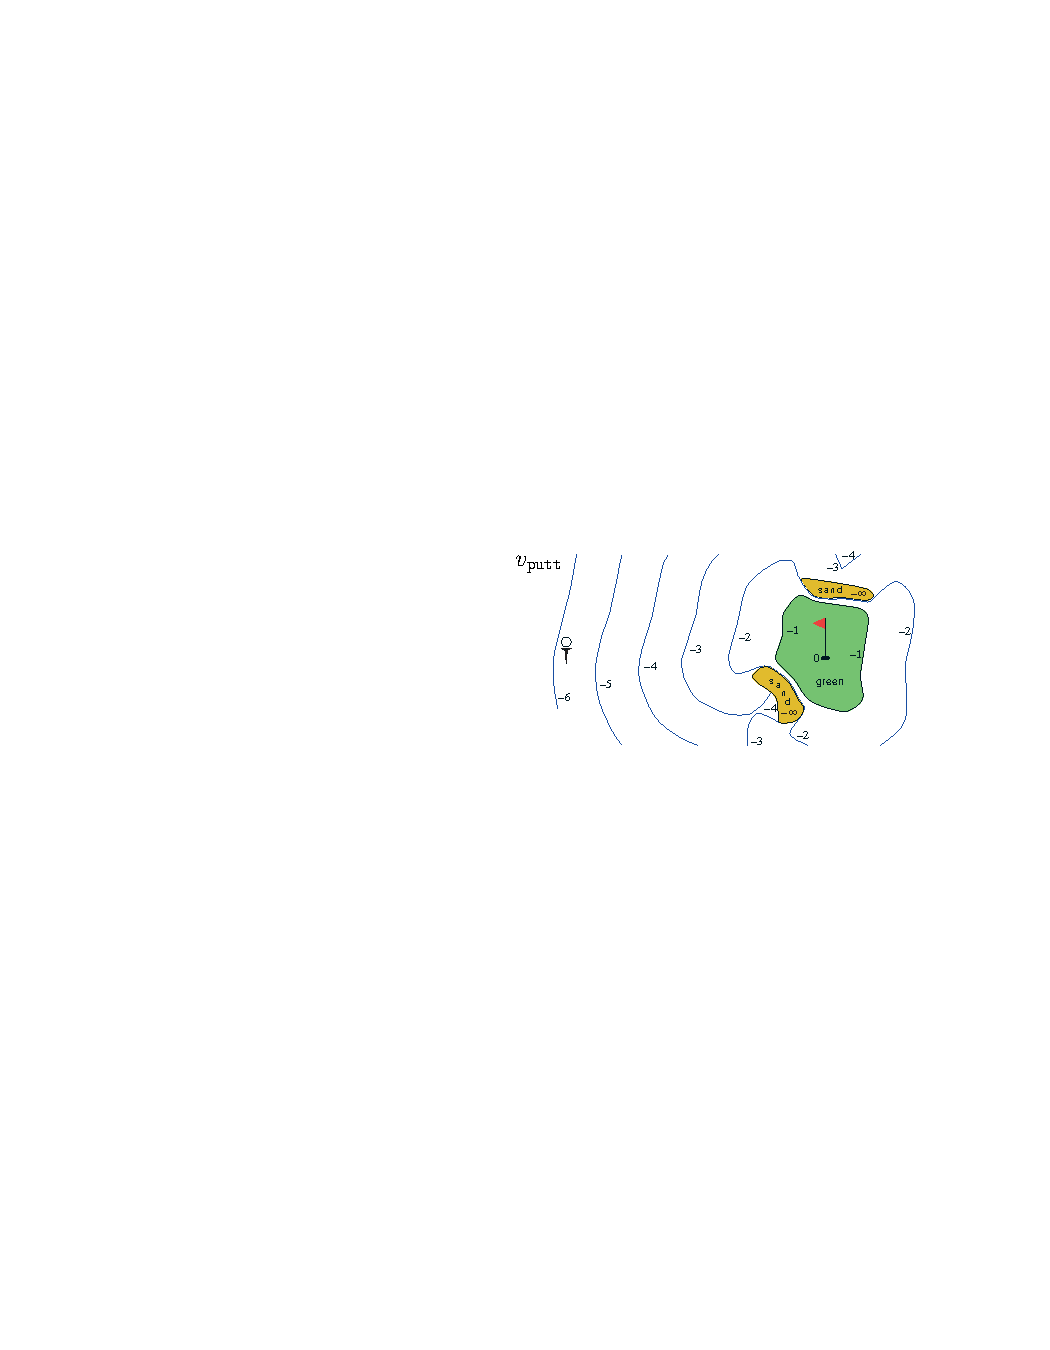
\includegraphics[width=6cm]{fig/lec02/Value_Golf.pdf}
	\caption{Isolines indicate state value of different golf ball locations (source: R. Sutton and G. Barto, Reinforcement learning: an introduction, 2018, \href{https://creativecommons.org/licenses/by-nc-nd/2.0/}{CC BY-NC-ND 2.0})}
	\label{fig:Value_Golf}
\end{figure}
}

%%%%%%%%%%%%%%%%%%%%%%%%%%%%%%%%%%%%%%%%%%%%%%%%%%%%%%%%%%%%%
%% State-Value Samples Forest Markov Reward Process %%
%%%%%%%%%%%%%%%%%%%%%%%%%%%%%%%%%%%%%%%%%%%%%%%%%%%%%%%%%%%%%
\frame{\frametitle{State-Value Samples of Forest MRP}
\begin{figure}		
	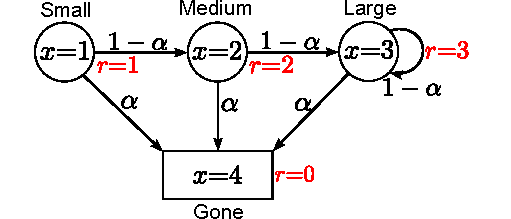
\includegraphics[width=8cm]{fig/lec02/Forest_Markov_Reward_Process.pdf}
\end{figure}
Exemplary \hl{samples} $\hat{v}$ with $\gamma=0.5$ starting in $x=1$:
\begin{alignat*}{2}
	&x=1 \rightarrow 4, &&\hat{v}= 1,\\ 
	&x=1 \rightarrow 2 \rightarrow 4, &&\hat{v}= 1 + 0.5\cdot 2=2.0,\\
	&x=1 \rightarrow 2 \rightarrow 3  \rightarrow 4, \quad&&\hat{v}=1+ 0.5\cdot 2+ 0.25\cdot 3=3.75,\\
	&x=1 \rightarrow 2 \rightarrow 3 \rightarrow 3 \rightarrow 4, \quad&&\hat{v}=1+ 0.5\cdot 2+0.25 \cdot 3+ 0.125\cdot3=4.13.
\end{alignat*}
}

%%%%%%%%%%%%%%%%%%%%%%%%%%%%%%%%%%%%%%%%%%%%%%%%%%%%%%%%%%%%%
%% Bellman Equation for MRPs (1)%%
%%%%%%%%%%%%%%%%%%%%%%%%%%%%%%%%%%%%%%%%%%%%%%%%%%%%%%%%%%%%%
\frame{\frametitle{Bellman Equation for MRPs (1)}
Problem: How to calculate all state values in closed form?\\ 
	\onslide<2->Solution: Bellman equation.
\begin{equation}
\onslide<3->{
\label{eq:Bellman_MRP}
\begin{split}
		v(x_k) &= \E{G_k|X_k=x_k}}\\
							&	\onslide<4->{= \E{R_{k+1} + \gamma R_{k+2} + \gamma^2 R_{k+3}+\ldots|X_k=x_k}}\\
							&\onslide<5->{= \E{R_{k+1} + \gamma \left(R_{k+2} + \gamma R_{k+3}+\ldots\right)|X_k=x_k}}\\
							&\onslide<6->{= \E{R_{k+1} + \gamma G_{k+1}|X_k=x_k}}\\
							&\onslide<7->{= \E{R_{k+1} + \gamma 	v(X_{k+1})|X_k=x_k}}
\end{split}
\end{equation}
\vspace*{\fill}
\onslide<8->{
\begin{figure}	
		 \hspace*{-1.5cm}
		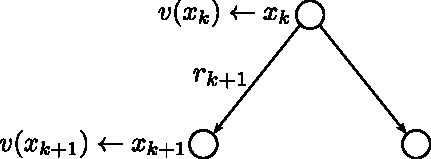
\includegraphics[width=6.1cm]{fig/lec02/Back_Up_MRP.pdf}
		\caption{Backup diagram for $v(x_k)$}
		\label{fig:Back_Up_MRP}
\end{figure}
}
}

%%%%%%%%%%%%%%%%%%%%%%%%%%%%%%%%%%%%%%%%%%%%%%%%%%%%%%%%%%%%%
%% Bellman Equation for MRPs (2) %%
%%%%%%%%%%%%%%%%%%%%%%%%%%%%%%%%%%%%%%%%%%%%%%%%%%%%%%%%%%%%%
\frame{\frametitle{Bellman Equation for MRPs (2)}
Assuming non-random rewards for every state $X=x\in\mathcal{X}$
\begin{equation}
	\bm{r}_{\mathcal{X}}= \begin{bmatrix} \mathcal{R}(x_1) & \cdots & \mathcal{R}(x_n)\end{bmatrix}\T = \begin{bmatrix} \mathcal{R}_1 & \cdots & \mathcal{R}_n\end{bmatrix}\T
\end{equation}
for a finite number of $n$ states with state-values
\begin{equation}
	\bm{v}_{\mathcal{X}}= \begin{bmatrix} v(x_1) & \cdots & v(x_n)\end{bmatrix}\T = \begin{bmatrix} v_1 & \cdots & v_n\end{bmatrix}\T
\end{equation}
one can derive a linear equation system based on \figref{fig:Back_Up_MRP}:\pause
\begin{equation}
\label{eq:Bellman_MRP_linear}
\begin{split}
	\bm{v}_{\mathcal{X}}&=\bm{r}_{\mathcal{X}}+\gamma\bm{\mathcal{P}}_{xx'}\bm{v}_{\mathcal{X}},\\
	\begin{bmatrix} v_1 \\ \vdots \\ v_n \end{bmatrix} &= \begin{bmatrix} \mathcal{R}_1 \\ \vdots \\ \mathcal{R}_n \end{bmatrix} + \gamma\begin{bmatrix} p_{11} & \cdots & p_{1n}\\ \vdots &  & \vdots\\ p_{n1} & \cdots & p_{nn}\end{bmatrix}\begin{bmatrix} v_1 \\ \vdots \\ v_n \end{bmatrix} .
\end{split}
\end{equation}
}

%%%%%%%%%%%%%%%%%%%%%%%%%%%%%%%%%%%%%%%%%%%%%%%%%%%%%%%%%%%%%
%% Sovling the MRP Bellman Equation %%
%%%%%%%%%%%%%%%%%%%%%%%%%%%%%%%%%%%%%%%%%%%%%%%%%%%%%%%%%%%%%
\frame{\frametitle{Solving the MRP Bellman Equation}
Above, \eqref{eq:Bellman_MRP_linear} is a normal equation in $\bm{v}_{\mathcal{X}}$:
\begin{equation}
\label{eq:MRP_normal_equation}
\begin{split}
\bm{v}_{\mathcal{X}}&=\bm{r}_{\mathcal{X}}+\gamma\bm{\mathcal{P}}_{xx'}\bm{v}_{\mathcal{X}},\\
\Leftrightarrow \underbrace{\left(\bm{I}-\gamma\bm{\mathcal{P}}_{xx'}\right)}_{\bm{A}}\underbrace{\bm{v}_{\mathcal{X}}}_{x}&=\underbrace{\bm{r}_{\mathcal{X}}}_{\bm{b}}.
\end{split}
\end{equation}
Possible solutions:
\begin{itemize}
	\item Direct inversion (Gaussian elimination, $\mathcal{O}(n^3)$)\pause
	\item Matrix decomposition (QR, Cholesky, etc. , $\mathcal{O}(n^3)$)\pause
	\item Iterative solutions (e.g., Krylov-subspaces, often better than $\mathcal{O}(n^3)$)\pause
\end{itemize}
\vspace{0.5cm}
In RL identifying and solving \eqref{eq:MRP_normal_equation} is a key task, which is often realized only approximately for high-order state spaces. 
}
%%%%%%%%%%%%%%%%%%%%%%%%%%%%%%%%%%%%%%%%%%%%%%%%%%%%%%%%%%%%%
%% Forest Markov Reward Process with State-Values%%
%%%%%%%%%%%%%%%%%%%%%%%%%%%%%%%%%%%%%%%%%%%%%%%%%%%%%%%%%%%%%
\frame{\frametitle{Example of a Markov Reward Process with State Values}
\begin{figure}		
	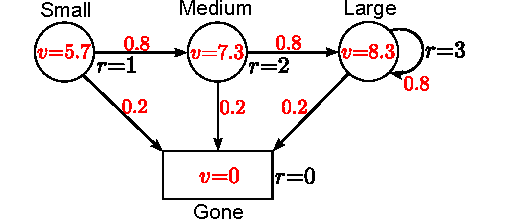
\includegraphics[width=10cm]{fig/lec02/Forest_Markov_Reward_Process_State_Value.pdf}
	\caption{Forest Markov reward process including state values}
	\label{fig:Forest_Markov_Chain_State_Value}
\end{figure}
\begin{itemize}
	\item Discount factor $\gamma=0.8$
	\item Disaster probability $\alpha=0.2$
\end{itemize}
}

%%%%%%%%%%%%%%%%%%%%%%%%%%%%%%%%%%%%%%%%%%%%%%%%%%%%%%%%%%%%%%%%%%
\section{Finite Markov Decision Processes} 
%%%%%%%%%%%%%%%%%%%%%%%%%%%%%%%%%%%%%%%%%%%%%%%%%%%%%%%%%%%%%%%%%%
\begin{frame}
\frametitle{Table of Contents}
\tableofcontents[currentsection]
\end{frame}

%%%%%%%%%%%%%%%%%%%%%%%%%%%%%%%%%%%%%%%%%%%%%%%%%%%%%%%%%%%%%
%% Markov Decision Process %%
%%%%%%%%%%%%%%%%%%%%%%%%%%%%%%%%%%%%%%%%%%%%%%%%%%%%%%%%%%%%%
\frame{\frametitle{Markov Decision Process}

\begin{defi}{Finite Markov decision process}{Markov_decision_process}
A \hl{finite Markov decision process (MDP)} is a tuple $\left\langle\mathcal{X}, \hl{\mathcal{U}}, \bm{\mathcal{P}}, \mathcal{R}, \gamma \right\rangle$ with
\begin{itemize}
	\item $\mathcal{X}$ being a finite set of discrete-time states $X_k\in\mathcal{X}$, 
	\item \hl{$\mathcal{U}$ as a finite set of discrete-time actions $U_k\in\mathcal{U}$,} 
	\item $\bm{\mathcal{P}}=\bm{\mathcal{P}}_{xx'}^{\hl{u}}$ is the state transition probability $\bm{\mathcal{P}}=\Pb{X_{k+1}=x'|X_{k}=x_k, \hl{U_{k}=u_k}}$,
	\item $\mathcal{R}$ is a reward function, $\mathcal{R}=\mathcal{R}_x^{\hl{u}}=\E{R_{k+1}|X_k=x_k, \hl{U_{k}=u_k}}$ and 
	\item $\gamma$ is a discount factor, $\gamma\in\left\{\mathbb{R}|0 \leq \gamma \leq 1\right\}$.
\end{itemize}
\end{defi}
\pause
\begin{itemize}
	\item Markov reward process is extended with actions / decisions.
	\item Now, rewards also depend on action $U_k$.
\end{itemize}
}

%%%%%%%%%%%%%%%%%%%%%%%%%%%%%%%%%%%%%%%%%%%%%%%%%%%%%%%%%%%%%
%% Forest Markov Decision Process (1) %%
%%%%%%%%%%%%%%%%%%%%%%%%%%%%%%%%%%%%%%%%%%%%%%%%%%%%%%%%%%%%%
\frame{\frametitle{Example of a Markov Decision Process (1)}
\begin{figure}		
	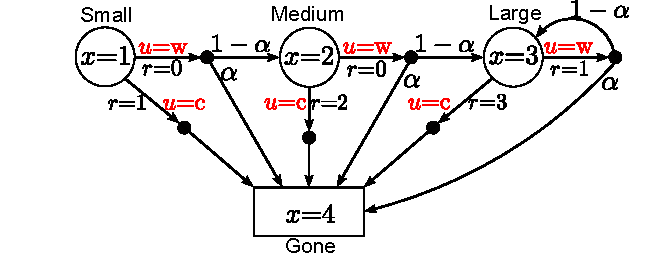
\includegraphics[width=11cm]{fig/lec02/Forest_Markov_Decision_Process.pdf}
	\caption{Forest Markov decision process}
	\label{fig:Forest_Markov_Decision_Process}
\end{figure}

\begin{itemize}
	\item Two actions possible in each state:
	\begin{itemize}
		\item Wait $u=w$: let the tree grow.
		\item Cut $u=c$: gather the wood.
	\end{itemize}
	\item With increasing tree size the wood reward increases as well.
\end{itemize}
}

%%%%%%%%%%%%%%%%%%%%%%%%%%%%%%%%%%%%%%%%%%%%%%%%%%%%%%%%%%%%%
%% Forest Markov Decision Process (2) %%
%%%%%%%%%%%%%%%%%%%%%%%%%%%%%%%%%%%%%%%%%%%%%%%%%%%%%%%%%%%%%
\frame{\frametitle{Example of a Markov Decision Process (2)}
For the previous example the state transition probability matrix and reward function are given as:
\begin{alignat*}{2}
	\bm{\mathcal{P}}_{xx'}^{u=c} &= \begin{bmatrix}0 & 0 & 0 & 1  \\ 0 & 0 &0 & 1 \\ 0 & 0 &0 & 1 \\ 0 & 0 & 0 & 1\end{bmatrix}, \quad \bm{\mathcal{P}}_{xx'}^{u=w} &&= \begin{bmatrix}0 & 1-\alpha & 0 & \alpha  \\ 0 & 0 &1-\alpha & \alpha \\ 0 & 0 &1-\alpha & \alpha \\ 0 & 0 & 0 & 1\end{bmatrix},\\
	\bm{r}_{\mathcal{X}}^{u=c} &= \begin{bmatrix}1 & 2 & 3 & 0 \end{bmatrix}\T, \quad \bm{r}_{\mathcal{X}}^{u=w} &&= \begin{bmatrix}0 & 0 & 1 & 0 \end{bmatrix}\T .
\end{alignat*}
\begin{itemize}
	\item The term $\bm{r}_{\mathcal{X}}^u$ is the abbreviated form for receiving the output of $\mathcal{R}$ for the entire state space $\mathcal{X}$ given the action $u$.
\end{itemize}
}

%%%%%%%%%%%%%%%%%%%%%%%%%%%%%%%%%%%%%%%%%%%%%%%%%%%%%%%%%%%%%
%% Policy (1) %%
%%%%%%%%%%%%%%%%%%%%%%%%%%%%%%%%%%%%%%%%%%%%%%%%%%%%%%%%%%%%%
\frame{\frametitle{Policy (1)}
\onslide<1->{
\begin{defi}{Policy in MDP (1)}{Policy_MDP}
In an MDP environment, a \hl{policy} is a distribution over actions given states:
\begin{equation}
\label{eq:Policy_MDP}
	\pi(u_k|x_k)=\Pb{U_k=u_k  | X_k=x_k}\, .
\end{equation}
\end{defi}
}
\vspace{-0.05cm}
\begin{itemize}
	\onslide<2->{\item In MDP, policies depend only on the current state.}
	\onslide<3->{\item A policy fully defines the agent's behavior.}
	\onslide<4->{\item Might relax to a deterministic policy for certain applications.} 
\end{itemize}
\onslide<1->{
\begin{figure}		
	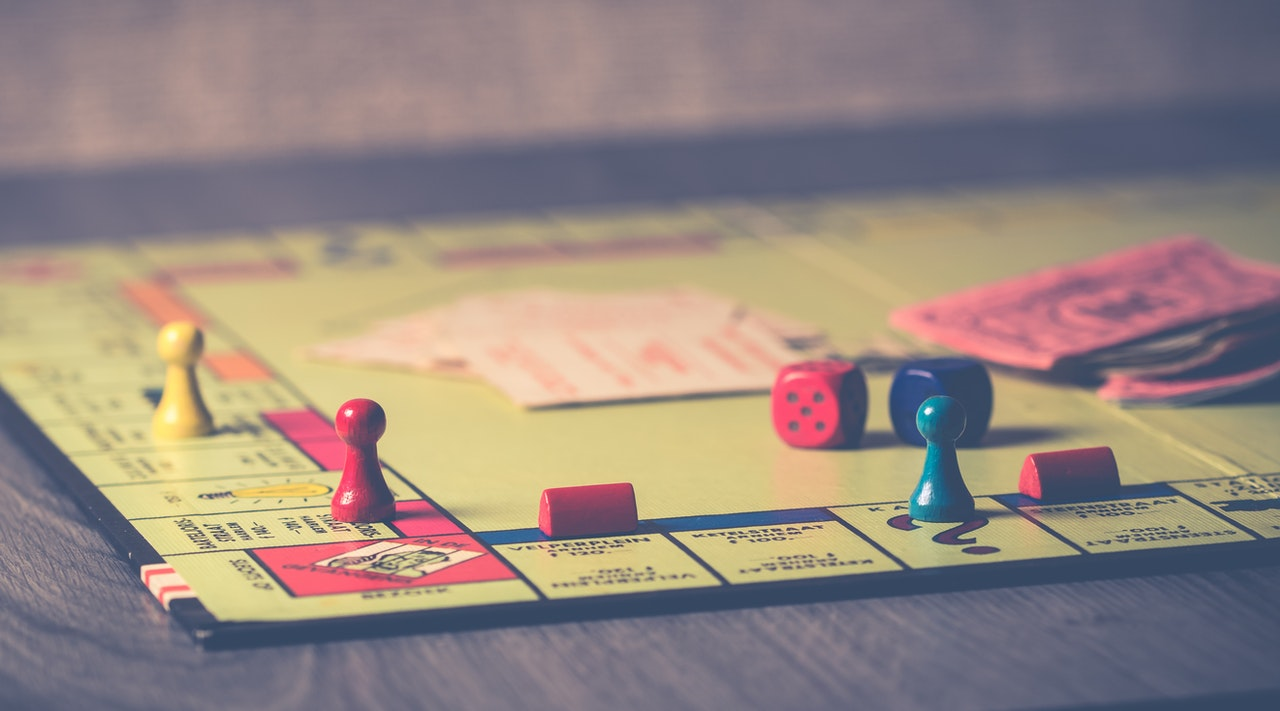
\includegraphics[width=5.75cm]{fig/lec02/monopoly.jpg}
	\caption{What is you best Monopoly policy? (source: Ylanite Koppens on \href{https://www.pexels.com/de-de/foto/begrifflich-brettspiel-drinnen-farben-776654/}{Pexels})}
\end{figure}
}
}

%%%%%%%%%%%%%%%%%%%%%%%%%%%%%%%%%%%%%%%%%%%%%%%%%%%%%%%%%%%%%
%% Policy (2) %%
%%%%%%%%%%%%%%%%%%%%%%%%%%%%%%%%%%%%%%%%%%%%%%%%%%%%%%%%%%%%%
\frame{\frametitle{Policy (2)}
Given an MDP $\left\langle\mathcal{X}, \mathcal{U}, \bm{\mathcal{P}}, \mathcal{R}, \gamma \right\rangle$ and a policy $\bm{\pi}$:
\begin{itemize}
	\item The state sequence $X_k, X_{k+1},\ldots$ is a Markov chain $\left\langle\mathcal{X}, \bm{\mathcal{P}}^{\pi} \right\rangle$ since the state transition probability is only depending on the state:
	\begin{equation}
		\bm{\mathcal{P}}_{xx'}^{\pi}=\sum_{u_k\in\mathcal{U}}\bm{\pi}(u_k|x_k)\bm{\mathcal{P}}_{xx'}^{u}\, .
	\end{equation}\pause
	\item Consequently, the sequence $X_k, R_{k+1}, X_{k+1},R_{k+2},\ldots$ of states and rewards is a Markov reward process $\left\langle\mathcal{X}, \bm{\mathcal{P}}^{\pi}, \mathcal{R}^{\pi}, \gamma \right\rangle$:
	\begin{equation}
		\mathcal{R}_{xx'}^{\pi}=\sum_{u_k\in\mathcal{U}}\bm{\pi}(u_k|x_k)\mathcal{R}_{x}^{u}\, .
	\end{equation}
\end{itemize}
}

%%%%%%%%%%%%%%%%%%%%%%%%%%%%%%%%%%%%%%%%%%%%%%%%%%%%%%%%%%%%%
%% Recap on Value functions %%
%%%%%%%%%%%%%%%%%%%%%%%%%%%%%%%%%%%%%%%%%%%%%%%%%%%%%%%%%%%%%
\frame{\frametitle{Recap on MDP Value Functions}

\begin{defi}{State-value function}{state_value_MDP}
The state-value function of an MDP is the expected return starting in $x_k$ following policy $\pi$:
\begin{equation*}
		v_\pi(x_k) = \El{G_k|X_k=x_k}{\pi}=\El{\left. \sum_{i=0}^\infty \gamma^i R_{k+i+1}\right|X_k}{\pi}\,.
	\end{equation*}
\end{defi}
\pause
\begin{defi}{Action-value function}{action_value_MDP}
The action-value function of an MDP is the expected return starting in $x_k$ taking action $u_k$ following policy $\pi$:
\begin{equation*}
		q_\pi(x_k,u_k) = \El{G_k|X_k=x_k, U_k=u_k}{\pi}=\El{\left.\sum_{i=0}^\infty \gamma^i R_{k+i+1}\right|X_k, U_k}{\pi}\, .
	\end{equation*}
\end{defi}
}

%%%%%%%%%%%%%%%%%%%%%%%%%%%%%%%%%%%%%%%%%%%%%%%%%%%%%%%%%%%%%
%% Bellman Expectation Equation (1) %%
%%%%%%%%%%%%%%%%%%%%%%%%%%%%%%%%%%%%%%%%%%%%%%%%%%%%%%%%%%%%%
\frame{\frametitle{Bellman Expectation Equation (1)}
Analog to \eqref{eq:Bellman_MRP}, the state value of an MDP can be decomposed into a Bellman notation:
\begin{equation}
	v_\pi(x_k)	= \El{R_{k+1} + \gamma 	v_{\pi}(X_{k+1})|X_k=x_k}{\pi}\, .
\end{equation}
\pause
In finite MDPs the state value can be directly linked to the action value (cf.~\figref{fig:Back_Up_Value_MDP}):
\begin{equation}
\label{eq:v_MDP_finite}
	v_\pi(x_k)	= \sum_{u_k\in\mathcal{U}}\pi(u_k|x_k)q_\pi(x_k,u_k) \, .
\end{equation}
\pause
\vspace{0.5cm}
\begin{figure}	
		 \hspace*{-1.5cm}
		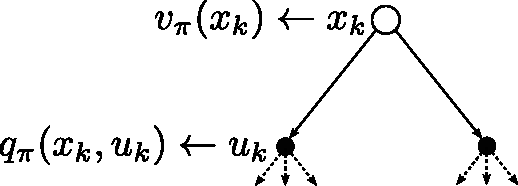
\includegraphics[width=6.5cm]{fig/lec02/Back_Up_Value_MDP.pdf}
		\caption{Backup diagram for $v_{\pi}(x_k)$}
		\label{fig:Back_Up_Value_MDP}
\end{figure}
}

%%%%%%%%%%%%%%%%%%%%%%%%%%%%%%%%%%%%%%%%%%%%%%%%%%%%%%%%%%%%%
%% Bellman Expectation Equation (2) %%
%%%%%%%%%%%%%%%%%%%%%%%%%%%%%%%%%%%%%%%%%%%%%%%%%%%%%%%%%%%%%
\frame{\frametitle{Bellman Expectation Equation (2)}
Likewise, the action value of an MDP can be decomposed into a Bellman notation:
\begin{equation}
	q_\pi(x_k,u_k)	= \El{R_{k+1} + \gamma 	q_{\pi}(X_{k+1},U_{k+1})|X_{k}=x_{k},U_{k}=u_{k}}{\pi}\, .
\end{equation}
\pause
In finite MDPs the action value can be directly linked to the state value (cf.~\figref{fig:Back_Up_Action_Value_MDP}):
\begin{equation}
\label{eq:q_MDP_finite}
	q_\pi(x_k,u_k)	= \mathcal{R}^u_x + \gamma \sum_{x_{k+1}\in\mathcal{X}}p_{xx'}^u v_\pi(x_{k+1}) \, .
\end{equation}
\pause
\vspace{0.5cm}
\begin{figure}	
		 \hspace*{-1.5cm}
		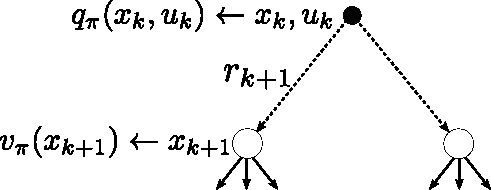
\includegraphics[width=6.5cm]{fig/lec02/Back_Up_Action_Value_MDP.pdf}
		\caption{Backup diagram for $q_{\pi}(x_k,u_k)$}
		\label{fig:Back_Up_Action_Value_MDP}
\end{figure}
}

%%%%%%%%%%%%%%%%%%%%%%%%%%%%%%%%%%%%%%%%%%%%%%%%%%%%%%%%%%%%%
%% Bellman Expectation Equation (3) %%
%%%%%%%%%%%%%%%%%%%%%%%%%%%%%%%%%%%%%%%%%%%%%%%%%%%%%%%%%%%%%
\frame{\frametitle{Bellman Expectation Equation (3)}
Inserting \eqref{eq:q_MDP_finite} into \eqref{eq:v_MDP_finite} directly results in:
\begin{equation}
	v_\pi(x_k)	= \sum_{u_k\in\mathcal{U}}\pi(u_k|x_k)\left(\mathcal{R}^u_x + \gamma\sum_{x_{k+1}\in\mathcal{X}}p_{xx'}^u v_\pi(x_{k+1})\right) \, .
\end{equation}
\pause
Conversely, the action value becomes:
\begin{equation}
	q_\pi(x_k,u_k)	= \mathcal{R}^u_x + \gamma\sum_{x_{k+1}\in\mathcal{X}}p_{xx'}^u \left(\sum_{u_{k+1}\in\mathcal{U}}\pi(u_{k+1}|x_{k+1})q_\pi(x_{k+1},u_{k+1})\right) \, .
\end{equation}
}

%%%%%%%%%%%%%%%%%%%%%%%%%%%%%%%%%%%%%%%%%%%%%%%%%%%%%%%%%%%%%
%% Bellman Expectation Equation in Matrix Form %%
%%%%%%%%%%%%%%%%%%%%%%%%%%%%%%%%%%%%%%%%%%%%%%%%%%%%%%%%%%%%%
\frame{\frametitle{Bellman Expectation Equation in Matrix Form}
Given a policy $\pi$ and following the same assumptions as for \eqref{eq:Bellman_MRP_linear}, the Bellman expectation equation can be expressed in Matrix form:
\begin{equation}
\label{eq:Bellman_MDP_linear}
\begin{split}
	\bm{v}_{\mathcal{X}}^{\pi}&=\bm{r}_{\mathcal{X}}^{\pi}+\gamma\bm{\mathcal{P}}_{xx'}^{\pi}\bm{v}_{\mathcal{X}}^{\pi},\\
	\begin{bmatrix} v_{1}^{\pi} \\ \vdots \\ v_{n}^{\pi} \end{bmatrix} &= \begin{bmatrix} \mathcal{R}_{1}^{\pi} \\ \vdots \\ \mathcal{R}_{n}^{\pi} \end{bmatrix} + \gamma\begin{bmatrix} p_{11}^{\pi} & \cdots & p_{1n}^{\pi}\\ \vdots &  & \vdots\\ p_{n1}^{\pi} & \cdots & p_{nn}^{\pi}\end{bmatrix}\begin{bmatrix} v_{1}^{\pi} \\ \vdots \\ v_{n}^{\pi} \end{bmatrix}.
\end{split}
\end{equation}
Here, $\bm{r}_{\mathcal{X}}^{\pi}$ and $\bm{\mathcal{P}}_{xx'}^{\pi}$ are the rewards and state transition probability following policy $\pi$. \pause Hence, the state value can be calculated by solving \eqref{eq:Bellman_MDP_linear} for $\bm{v}_{\mathcal{X}}^{\pi}$, e.g., by direct matrix inversion:
\begin{equation}
	\bm{v}_{\mathcal{X}}^{\pi}=\left(\bm{I}-\gamma\bm{\mathcal{P}}_{xx'}^{\pi}\right)^{-1}\bm{r}_{\mathcal{X}}^{\pi}.
\end{equation}
}

%%%%%%%%%%%%%%%%%%%%%%%%%%%%%%%%%%%%%%%%%%%%%%%%%%%%%%%%%%%%%
%% Bellman Expectation Equation Applied to Forest Tree Example (1)%%
%%%%%%%%%%%%%%%%%%%%%%%%%%%%%%%%%%%%%%%%%%%%%%%%%%%%%%%%%%%%%
\frame{\frametitle{Bellman Expectation Equation \& Forest Tree Example (1)}
Let's assume following very simple policy ('\textit{fifty-fifty}')
\begin{equation*}
\pi(u = \mbox{cut}|x) = 0.5, \quad \pi(u = \mbox{wait}|x) = 0.5 \quad\forall x\in\mathcal{X} \, .
\end{equation*}
\pause
Applied to the given environment behavior
\begin{alignat*}{2}
	\bm{\mathcal{P}}_{xx'}^{u=c} &= \begin{bmatrix}0 & 0 & 0 & 1  \\ 0 & 0 &0 & 1 \\ 0 & 0 &0 & 1 \\ 0 & 0 & 0 & 1\end{bmatrix}, \quad \bm{\mathcal{P}}_{xx'}^{u=w} &&= \begin{bmatrix}0 & 1-\alpha & 0 & \alpha  \\ 0 & 0 &1-\alpha & \alpha \\ 0 & 0 &1-\alpha & \alpha \\ 0 & 0 & 0 & 1\end{bmatrix},\\
	\bm{r}_{\mathcal{X}}^{u=c} &= \begin{bmatrix}1 & 2 & 3 & 0 \end{bmatrix}\T, \quad \bm{r}_{\mathcal{X}}^{u=w} &&= \begin{bmatrix}0 & 0 & 1 & 0 \end{bmatrix}\T ,
\end{alignat*}
\pause
one receives:
\begin{equation*}
	\bm{\mathcal{P}}_{xx'}^{\pi} = \begin{bmatrix}0 & \frac{1-\alpha}{2} & 0 & \frac{1+\alpha}{2}  \\ 0 & 0 &\frac{1-\alpha}{2} & \frac{1+\alpha}{2} \\ 0 & 0 &\frac{1-\alpha}{2} & \frac{1+\alpha}{2} \\ 0 & 0 & 0 & 1\end{bmatrix}, \quad\bm{r}_{\mathcal{X}}^{\pi} = \begin{bmatrix}0.5 \\ 1 \\ 2 \\ 0 \end{bmatrix} .
\end{equation*}
}

%%%%%%%%%%%%%%%%%%%%%%%%%%%%%%%%%%%%%%%%%%%%%%%%%%%%%%%%%%%%%
%% Bellman Expectation Equation Applied to Forest Tree Example (2)%%
%%%%%%%%%%%%%%%%%%%%%%%%%%%%%%%%%%%%%%%%%%%%%%%%%%%%%%%%%%%%%
\frame{\frametitle{Bellman Expectation Equation \& Forest Tree Example (2)}
\begin{figure}		
	%\hspace*{-1.5cm}
	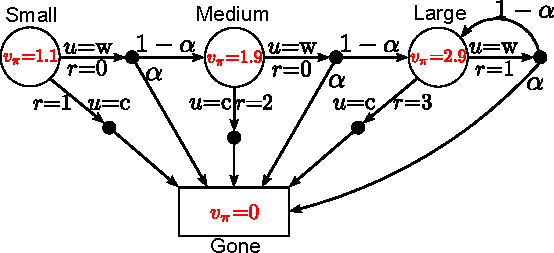
\includegraphics[width=10cm]{fig/lec02/Forest_Markov_Decision_Process_State_Value.pdf}
	\caption{Forest MDP with fifty-fifty-policy including state values}
	\label{fig:Forest_Markov_Decision_Process_State_Value}
\end{figure}
\begin{itemize}
	\item Discount factor $\gamma=0.8$
	\item Disaster probability $\alpha=0.2$
\end{itemize}
}

%%%%%%%%%%%%%%%%%%%%%%%%%%%%%%%%%%%%%%%%%%%%%%%%%%%%%%%%%%%%%
%% Bellman Expectation Equation Applied to Forest Tree Example (3)%%
%%%%%%%%%%%%%%%%%%%%%%%%%%%%%%%%%%%%%%%%%%%%%%%%%%%%%%%%%%%%%
\frame{\frametitle{Bellman Expectation Equation \& Forest Tree Example (3)}
Using the Bellman expectation eq. \eqref{eq:q_MDP_finite} the action values can be directly calculated: 
\vspace{0.5cm}
\begin{figure}		
	\hspace*{0.5cm}
	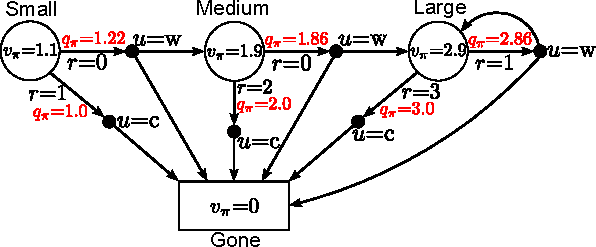
\includegraphics[width=10cm]{fig/lec02/Forest_Markov_Decision_Process_Action_Value.pdf}
	\caption{Forest MDP with fifty-fifty-policy plus action values}
	\label{fig:Forest_Markov_Decision_Process_Action_Value}
\end{figure}
Is the '\textit{fifty-fifty-policy}' maximizing our long-term reward? How can you evaluate your answer?
}

%%%%%%%%%%%%%%%%%%%%%%%%%%%%%%%%%%%%%%%%%%%%%%%%%%%%%%%%%%%%%%%%%%
\section{Optimal Policies and Value Functions} 
%%%%%%%%%%%%%%%%%%%%%%%%%%%%%%%%%%%%%%%%%%%%%%%%%%%%%%%%%%%%%%%%%%
\begin{frame}
\frametitle{Table of Contents}
\tableofcontents[currentsection]
\end{frame}

%%%%%%%%%%%%%%%%%%%%%%%%%%%%%%%%%%%%%%%%%%%%%%%%%%%%%%%%%%%%%
%% Optimal Value Functions in MDP %%
%%%%%%%%%%%%%%%%%%%%%%%%%%%%%%%%%%%%%%%%%%%%%%%%%%%%%%%%%%%%%
\frame{\frametitle{Optimal Value Functions in an MDP}
\begin{defi}{Optimal state-value function}{optimal_state_value_MDP}
The optimal state-value function of an MDP is the maximum state-value function over all polices:
\begin{equation}
		v^*(x) = \max_{\pi} v_{\pi}(x)\,.
	\end{equation}
\end{defi}
\vspace{-0.2cm}
\pause
\begin{defi}{Optimal action-value function}{optimal_action_value_MDP}
The optimal action-value function of an MDP is the maximum action-value function over all polices:
\begin{equation}
		q^*(x,u) = \max_{\pi} q_\pi(x,u)\, .
	\end{equation}
\end{defi}
\vspace{-0.1cm}
\pause
\begin{itemize}
	\item The optimal value function denotes the best possible agent's performance for a given MDP / environment. \pause
	\item A (finite) MDP can be easily solved in an optimal way if $q^*(x,u)$ is known. 
\end{itemize}
}

%%%%%%%%%%%%%%%%%%%%%%%%%%%%%%%%%%%%%%%%%%%%%%%%%%%%%%%%%%%%%
%% Optimal Policy in MDP %%
%%%%%%%%%%%%%%%%%%%%%%%%%%%%%%%%%%%%%%%%%%%%%%%%%%%%%%%%%%%%%
\frame{\frametitle{Optimal Policy in an MDP}
Define a partial ordering over polices
\begin{equation}
	\pi \geq \pi' \quad \mbox{if} \quad v_{\pi}(x) \geq v_{\pi'}(x) \quad \forall x\in\mathcal{X} \,.
\end{equation}
\pause
\begin{theo}{Optimal policies in MDPs}{Optimal_policies_MDP}
For any finite MDP
\begin{itemize}
	\item there exists an optimal policy $\pi^*\geq\pi$ that is better or equal to all other policies,
	\item all optimal policies achieve the same optimal state-value function $v^*(x)=v_{\pi^*}(x)$,
	\item all optimal policies achieve the same optimal action-value function $q^*(x, u)=q_{\pi^*}(x, u)$.
\end{itemize}
\end{theo}
}

%%%%%%%%%%%%%%%%%%%%%%%%%%%%%%%%%%%%%%%%%%%%%%%%%%%%%%%%%%%%%
%% Bellman Optimality Equation (1)%%
%%%%%%%%%%%%%%%%%%%%%%%%%%%%%%%%%%%%%%%%%%%%%%%%%%%%%%%%%%%%%
\frame{\frametitle{Bellman Optimality Equation (1)}
\onslide<1->{
\begin{theo}{Bellman's principle of optimality}{bellman_principle_optimality}
``\textit{An optimal policy has the property that whatever the initial state and initial decision are, the remaining decisions must constitute an optimal policy with regard to the state resulting from the first decision.}''(R.E. Bellman, Dynamic Programming, 1957) 
\end{theo}
}
\begin{itemize}
	\onslide<2->{\item Any policy (i.e., also the optimal one) must satisfy the self-consistency condition given by the Bellman expectation equation.}
	\onslide<3->{\item An optimal policy must equal the expected return for the best action of a given state:}
\end{itemize}
\onslide<4->{
\begin{equation}
\begin{split}
		v^*(x_k) &= \max_{u} q_{\pi^*}(x_k, u)\, ,}\\
									&\onslide<5->{= \max_{u} \El{G_k|X_k=x_k, U=u}{\pi^*}\, ,}\\
									&\onslide<6->{= \max_{u} \El{R_{k+1} + \gamma G_{k+1}|X_k=x_k, U=u}{\pi^*}\, ,}\\
									&\onslide<7->{= \max_{u} \E{R_{k+1} + \gamma v^*(X_{k+1})|X_k=x_k, U=u}\, .}
\end{split}
\end{equation}
}

%%%%%%%%%%%%%%%%%%%%%%%%%%%%%%%%%%%%%%%%%%%%%%%%%%%%%%%%%%%%%
%% Bellman Optimality Equation (2)%%
%%%%%%%%%%%%%%%%%%%%%%%%%%%%%%%%%%%%%%%%%%%%%%%%%%%%%%%%%%%%%
\frame{\frametitle{Bellman Optimality Equation (2)}
Again, the Bellman optimality equation can be visualized by a backup diagram: 
\begin{figure}	
		 %\hspace*{-1.5cm}
		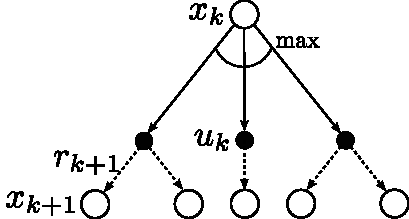
\includegraphics[width=4.5cm]{fig/lec02/Back_Up_Value_Optimal_MDP.pdf}
		\caption{Backup diagram for $v^*(x_k)$}
		\label{fig:Back_Up_Value_Optimal_MDP}
\end{figure}
\pause
For a finite MDP the following expression results:
\begin{equation}
\label{eq:Bellman_Optimal_State_Value_MDP}
	v^*(x_k) = \max_{u_k}\, \mathcal{R}^u_x+ \gamma \sum_{x_{k+1}\in\mathcal{X}}p_{xx'}^u v_{\pi^*}(x_{k+1}) .
\end{equation}
}

%%%%%%%%%%%%%%%%%%%%%%%%%%%%%%%%%%%%%%%%%%%%%%%%%%%%%%%%%%%%%
%% Bellman Optimality Equation (3)%%
%%%%%%%%%%%%%%%%%%%%%%%%%%%%%%%%%%%%%%%%%%%%%%%%%%%%%%%%%%%%%
\frame{\frametitle{Bellman Optimality Equation (3)}
Likewise, the Bellman optimality equation is applicable to the action value:
\begin{equation}
	q^*(x_k,u_k) = \E{R_{k+1}+ \gamma \max_{u_{k+1}} q^*(X_{k+1},U_{k+1})|X_k=x_k, U_k=u_k} . 
\end{equation}
\pause
And, in the finite MDP case:
\begin{equation}
\label{eq:Bellman_Optimal_action_Value_MDP}
	q^*(x_k,u_k) = \mathcal{R}^u_x + \gamma \sum_{x_{k+1}\in\mathcal{X}}p_{xx'}^u \max_{u_{k+1}}q^*(x_{k+1}, u_{k+1}) .
\end{equation}
\pause
\begin{figure}	
		 %\hspace*{-1.5cm}
		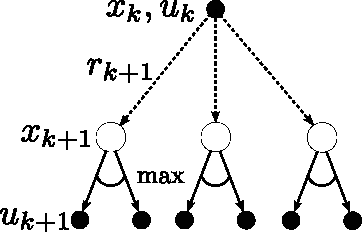
\includegraphics[width=4.7cm]{fig/lec02/Back_Up_Action_Value_Optimal_MDP.pdf}
		\caption{Backup diagram for $q^*(x_k,u_k)$}
		\label{fig:Back_Up_Action_Value_Optimal_MDP}
\end{figure}
}

%%%%%%%%%%%%%%%%%%%%%%%%%%%%%%%%%%%%%%%%%%%%%%%%%%%%%%%%%%%%%
%% Solving the Bellman Optimality Equation %%
%%%%%%%%%%%%%%%%%%%%%%%%%%%%%%%%%%%%%%%%%%%%%%%%%%%%%%%%%%%%%
\frame{\frametitle{Solving the Bellman Optimality Equation}
\begin{itemize}
	\item In finite MDPs with $n$ states, \eqref{eq:Bellman_Optimal_State_Value_MDP} delivers an \hl{algebraic equation system} with $n$ unknowns and $n$ \hl{state-value equations}. \pause
	\item Likewise, \eqref{eq:Bellman_Optimal_action_Value_MDP} delivers an algebraic equation system with up to $n\cdot m$ unknowns and $n \cdot m$ \hl{action-value equations} ($m=$number of actions). \pause
	\item Due to $\max$ operator the equation set is generally \hl{nonlinear}. Direct, closed form solution rarely available. \pause
	\item Hence, often  approximate / iterative solutions are required (upcoming lectures).\pause
	\item If environment is exactly known, solving for $v^*$ or $q^*$ directly delivers optimal policy. 
	\begin{itemize}
		\item If $v(x)$ is known, a one-step-ahead search is required to get $q(x)$.
		\item If $q(x, u)$ is known, directly choose $q^*$. \pause
	\end{itemize}
	\item Even though above decisions are very short sighted (one-step-ahead search for $v$ or direct choice of $q$), by Bellman's principle of optimality one receives the long-term maximum of the expected reward.
\end{itemize}
}

%%%%%%%%%%%%%%%%%%%%%%%%%%%%%%%%%%%%%%%%%%%%%%%%%%%%%%%%%%%%%
%% Optimal Forest MDP %%
%%%%%%%%%%%%%%%%%%%%%%%%%%%%%%%%%%%%%%%%%%%%%%%%%%%%%%%%%%%%%
\frame{\frametitle{Optimal Policy for Forest Tree MDP}
Remember the forest tree MDP example:
\begin{figure}		
	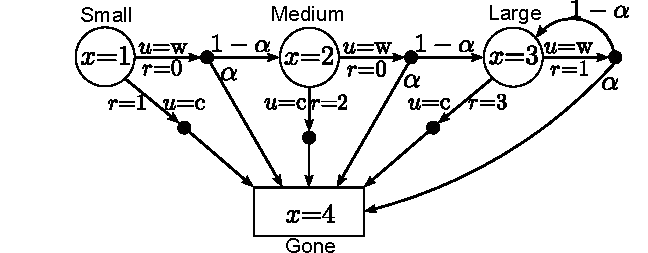
\includegraphics[width=11cm]{fig/lec02/Forest_Markov_Decision_Process_No_Color.pdf}
	\label{fig:Forest_Markov_Decision_Process_No_Color}
\end{figure}

\begin{itemize}
	\item Two actions possible in each state:
	\begin{itemize}
		\item Wait $u=w$: let the tree grow.
		\item Cut $u=c$: gather the wood.
	\end{itemize}
	\item Lets first calculate $v^*(x)$ and then $q^*(x,u)$.
\end{itemize}
}

%%%%%%%%%%%%%%%%%%%%%%%%%%%%%%%%%%%%%%%%%%%%%%%%%%%%%%%%%%%%%
%% Optimal Policy for Forest Tree MDP: State-Value (1)%%
%%%%%%%%%%%%%%%%%%%%%%%%%%%%%%%%%%%%%%%%%%%%%%%%%%%%%%%%%%%%%
\frame{\frametitle{Optimal Policy for Forest Tree MDP: State Value (1)}
\onslide<1->{Start with $v(x=4)$ ('gone') and then continue going backwards:}
\onslide<2->{
\begin{align*}
	v^*(x=4) &= 0\, ,}\\
	\onslide<3->{v^*(x=3) &= \max \begin{cases} 1 + \gamma\left[(1-\alpha)v^*(x=3) + \alpha v^*(x=4)\right]\, ,\\ 3+\gamma v^*(x=4)\, ,\end{cases}}\\
					 &\onslide<4->{= \max \begin{cases} 1 + \gamma\left[(1-\alpha)v^*(x=3)\right]\, ,\\ 3\, ,\end{cases}}\\\
	\onslide<5->{v^*(x=2) &= \max \begin{cases} 0 + \gamma\left[(1-\alpha)v^*(x=3) + \alpha v^*(x=4)\right]\, ,\\ 2+\gamma v^*(x=4)\, ,\end{cases}}\\
					 &\onslide<6->{= \max \begin{cases} \gamma\left[(1-\alpha)v^*(x=3)\right]\, ,\\ 2\, ,\end{cases}}\\
	\onslide<7->{v^*(x=1) &= \max \begin{cases} \gamma\left[(1-\alpha)v^*(x=2)\right]\, ,\\ 1\, .\end{cases}}
\end{align*}
}

%%%%%%%%%%%%%%%%%%%%%%%%%%%%%%%%%%%%%%%%%%%%%%%%%%%%%%%%%%%%%
%% Optimal Policy for Forest Tree MDP: State-Value (2)%%
%%%%%%%%%%%%%%%%%%%%%%%%%%%%%%%%%%%%%%%%%%%%%%%%%%%%%%%%%%%%%
\frame{\frametitle{Optimal Policy for Forest Tree MDP: State Value (2)}
\begin{itemize}
	\item Due to presence of terminal state ($x=4$) only three unknowns
	\item Solution: numerical optimization approach (e.g., simplex method, gradient descent,...)
\end{itemize}
\begin{figure}		
	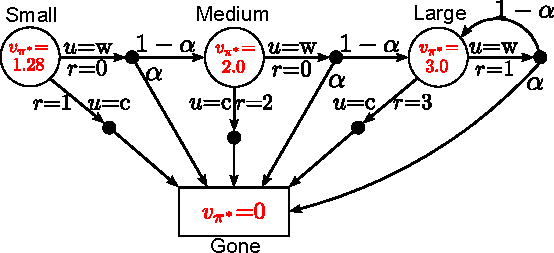
\includegraphics[width=11cm]{fig/lec02/Forest_Markov_Decision_Process_Optimal_State_Value.pdf}
		\caption{State values under optimal policy ($\gamma=0.8$,	$\alpha=0.2$)}
	\label{fig:Forest_Markov_Decision_Process_Optimal_State_Value}
\end{figure}
}

%%%%%%%%%%%%%%%%%%%%%%%%%%%%%%%%%%%%%%%%%%%%%%%%%%%%%%%%%%%%%
%% Optimal Policy for Forest Tree MDP: State-Value (3)%%
%%%%%%%%%%%%%%%%%%%%%%%%%%%%%%%%%%%%%%%%%%%%%%%%%%%%%%%%%%%%%
\frame{\frametitle{Optimal Policy for Forest Tree MDP: State Value (3)}
\begin{figure}		
	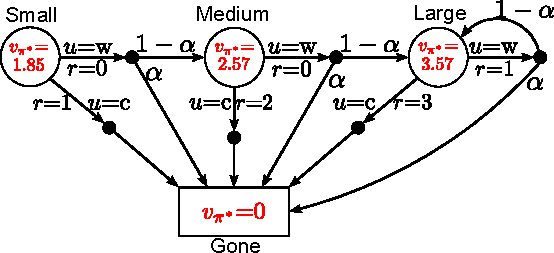
\includegraphics[width=11cm]{fig/lec02/Forest_Markov_Decision_Process_Optimal_State_Value_Gamma09.pdf}
		\caption{State values under optimal policy (\hl{$\gamma=0.9$},	$\alpha=0.2$)}
	\label{fig:Forest_Markov_Decision_Process_Optimal_State_Value_Gamma09}
\end{figure}
}

%%%%%%%%%%%%%%%%%%%%%%%%%%%%%%%%%%%%%%%%%%%%%%%%%%%%%%%%%%%%%
%% Optimal Policy for Forest Tree MDP: Action-Value (1)%%
%%%%%%%%%%%%%%%%%%%%%%%%%%%%%%%%%%%%%%%%%%%%%%%%%%%%%%%%%%%%%
\frame{\frametitle{Optimal Policy for Forest Tree MDP: Action Value (1)}
\onslide<1->{Use $u_{k+1}=u'$ to set up equation system:
\begin{align*}
q^*(x=1,u=c) &= 1\, ,}\\
\onslide<2->{q^*(x=1,u=w) &= \gamma(1-\alpha)\max_{u'}q^*(x=2,u')\, ,}\\
\onslide<3->{q^*(x=2,u=c) &= 2\, ,}\\
\onslide<4->{q^*(x=2,u=w) &= \gamma(1-\alpha)\max_{u'}q^*(x=3,u')\, ,}\\
\onslide<5->{q^*(x=3,u=c) &= 3\, ,}\\
\onslide<6->{q^*(x=3,u=w) &= 1+\gamma(1-\alpha)\max_{u'}q^*(x=3,u')\, .}
\end{align*}
\onslide<7->{
\begin{itemize}
	\item There are six action-state pairs in total.
	\item Three of them can be directly determined.
	\item Three unknowns and three equations remain.
\end{itemize}
}
}

%%%%%%%%%%%%%%%%%%%%%%%%%%%%%%%%%%%%%%%%%%%%%%%%%%%%%%%%%%%%%
%% Optimal Policy for Forest Tree MDP: Action-Value (2)%%
%%%%%%%%%%%%%%%%%%%%%%%%%%%%%%%%%%%%%%%%%%%%%%%%%%%%%%%%%%%%%
\frame{\frametitle{Optimal Policy for Forest Tree MDP: Action Value (2)}
\onslide<1->{
Rearrange $\max$ expressions for unknown action values: 
\begin{align*}
q^*(x=1,u=w) &= \gamma(1-\alpha)\max\begin{cases}\gamma(1-\alpha)\max\begin{cases}1+\gamma(1-\alpha)q^*(3,w)\\3\end{cases}\\2\end{cases}}\\
\onslide<2->{q^*(x=2,u=w) &= \gamma(1-\alpha)\max\begin{cases}1+\gamma(1-\alpha)q^*(3,w)\\3\end{cases}}\\
\onslide<3->{q^*(x=3,u=w) &= 1+\gamma(1-\alpha)\max\begin{cases}q^*(3,w)\\3\end{cases}\, .}
\end{align*}
\onslide<4->{Again, retrieve unknown optimal action values by numerical optimization solvers.}
}

%%%%%%%%%%%%%%%%%%%%%%%%%%%%%%%%%%%%%%%%%%%%%%%%%%%%%%%%%%%%%
%% Optimal Policy for Forest Tree MDP: Action-Value (3)%%
%%%%%%%%%%%%%%%%%%%%%%%%%%%%%%%%%%%%%%%%%%%%%%%%%%%%%%%%%%%%%
\frame{\frametitle{Optimal Policy for Forest Tree MDP: Action Value (3)}
\begin{figure}		
	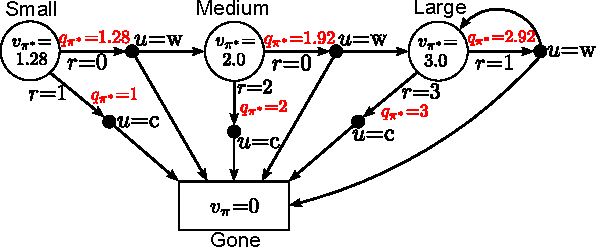
\includegraphics[width=11cm]{fig/lec02/Forest_Markov_Decision_Process_Optimal_Action_Value.pdf}
		\caption{Action values under optimal policy ($\gamma=0.8$,	$\alpha=0.2$)}
	\label{fig:Forest_Markov_Decision_Process_Optimal_Action_Value}
\end{figure}
}

%%%%%%%%%%%%%%%%%%%%%%%%%%%%%%%%%%%%%%%%%%%%%%%%%%%%%%%%%%%%%
%% Optimal Policy for Forest Tree MDP: Action-Value (4)%%
%%%%%%%%%%%%%%%%%%%%%%%%%%%%%%%%%%%%%%%%%%%%%%%%%%%%%%%%%%%%%
\frame{\frametitle{Optimal Policy for Forest Tree MDP: Action Value (4)}
\begin{figure}		
	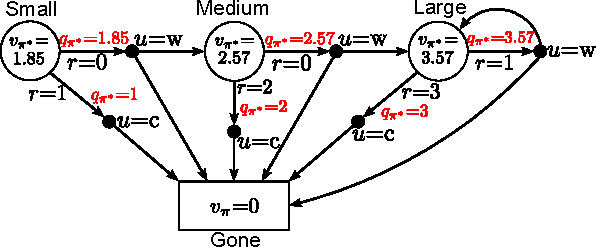
\includegraphics[width=11cm]{fig/lec02/Forest_Markov_Decision_Process_Optimal_Action_Value_Gamma09.pdf}
		\caption{Action values under optimal policy (\hl{$\gamma=0.9$},	$\alpha=0.2$)}
	\label{fig:Forest_Markov_Decision_Process_Optimal_Action_Value_Gamma09}
\end{figure}
}

%%%%%%%%%%%%%%%%%%%%%%%%%%%%%%%%%%%%%%%%%%%%%%%%%%%%%%%%%%%%%
%% Solving an MDP by Calculating Optimal State and Action-Values%%
%%%%%%%%%%%%%%%%%%%%%%%%%%%%%%%%%%%%%%%%%%%%%%%%%%%%%%%%%%%%%
\frame{\frametitle{Direct Numerical State and Action-Value Calculation}
\begin{itemize}
	\item Possible only for \hl{small action and state-space} MDPs
	\begin{itemize}
		\item 'Solving' Backgammon with $\approx 10^{20}$ states?
	\end{itemize}
	\pause
	\item Another issue: initial values?\pause
	\item And yet another issue: \hl{nonlinear system with multiple unknowns}
		\begin{itemize}
			\item Local solvers = local solutions
			\item Initial-point-dependent 
		\end{itemize}
		\pause
		\item And finally: total \hl{environment knowledge} required
\end{itemize}
\pause
\begin{block}{Framing the reinforcement learning problem}
Facing the above issues, RL addresses mainly two topics:
\begin{itemize}
	\item Approximate solutions of complex decision problems.
	\item Learning of such approximations based on environment interactions.
\end{itemize}
 
\end{block}
}

%%%%%%%%%%%%%%%%%%%%%%%%%%%%%%%%%%%%%%%%%%%%%%%%%%%%%%%%%%%%%
%% Summary %%
%%%%%%%%%%%%%%%%%%%%%%%%%%%%%%%%%%%%%%%%%%%%%%%%%%%%%%%%%%%%%
\begin{frame}
\frametitle{Summary: What You've Learned Today}
\begin{itemize}
	\item Differentiate finite Markov process models with or w/o rewards and actions.\pause
	\item Interpret such stochastic processes as simplified abstractions of real-world problems.\pause
	\item Understand the importance of value functions to describe the agent's performance. \pause
	\item Formulate value-function equation systems by the Bellman principle.\pause
	\item Recognize optimal policies.\pause
	\item Setting up nonlinear equation systems for retrieving optimal policies by the Bellman principle.\pause
	\item Solving for different value functions in MRP/MDP contexts by numerical optimization.
\end{itemize}
\end{frame}

%%%%%%%%%%%%%%%%%%%%%%%%%%%%%%%%%%%%%%%%%%%%%%%%%%%%%%%%%%%%%
%% Final Slide %%
%%%%%%%%%%%%%%%%%%%%%%%%%%%%%%%%%%%%%%%%%%%%%%%%%%%%%%%%%%%%%
\frame{\frametitle{The End for Today}
\begin{figure}

\includegraphics[width=10cm]{fig/lec02/dilbert.png}
\end{figure}
\vspace{1cm}
\centering
Thanks for your attention and have a nice week!
}
